\documentclass[11pt,a4paper]{article}
\usepackage{fontspec}
\setmainfont{TeX Gyre Pagella}
\newfontfamily\headfont{Inter}[UprightFont=*-ExtraBold,BoldFont=*-ExtraBold,Extension=.otf,Path=/usr/share/fonts/opentype/inter/]
\usepackage[a4paper,margin=2.3cm]{geometry}
\usepackage{graphicx,booktabs,float,caption,array,xcolor}
\usepackage[hidelinks]{hyperref}
\usepackage{titlesec}
\usepackage[round]{natbib}
\usepackage{setspace}
\setstretch{1.05}
\renewcommand{\topfraction}{0.9}
\renewcommand{\bottomfraction}{0.8}
\renewcommand{\textfraction}{0.1}
\renewcommand{\floatpagefraction}{0.75}
\setlength{\parindent}{0pt}
\setlength{\parskip}{0.55em}
\titleformat{\section}{\headfont\Large}{\thesection}{0.8em}{}
\titleformat{\subsection}{\headfont\large}{\thesubsection}{0.8em}{}
\captionsetup{font=small,labelfont=bf}
\urlstyle{same}
\hypersetup{pdftitle={The Internet's Seabed: Submarine Cables, When They Were Laid, Who Owns Them and Where They Crowd Together},pdfauthor={Tristan Hotham}}

\begin{document}
\begin{center}
{\Large\bfseries The Internet's Seabed\par}
\vspace{0.4em}
{\large Submarine cables, when they were laid, who owns them\\and where they crowd together\par}
\vspace{1.2em}
{\large Tristan Hotham\par}
\vspace{0.3em}
{\small Independent researcher\\
ORCID: 0000-0003-4931-9349\\
DOI: \detokenize{10.5281/zenodo.23856607}\par}
\vspace{0.8em}
2026
\end{center}

\begin{quote}
\small
\begin{center}\textbf{Abstract}\end{center}
Almost all intercontinental internet traffic travels through fibre-optic cables on the sea floor. I describe the network as recorded in TeleGeography's Submarine Cable Map, the most widely used open record of it, in its 2026 version: 608 cables in service with a combined length of 1,592,824 km and 105 planned cables with 502,770 km more, landing at 1,928 points in 186 countries and territories. I ask three questions. When was each cable laid? The ready-for-service years show two booms: the dot-com bubble, when 74 of today's cables came into service in 1999 to 2001, and the present, with a record 32 new cables in 2023 and 49 planned for 2027. Who owns the new cables? Matching owner names shows that Google, Meta, Amazon and Microsoft part-own none of the length ready before 2010, 24\% of the length ready in 2015 to 2019, 50\% in 2020 to 2026 and 55\% of the planned length. Where does the network squeeze through? Counting cables whose routes cross bands drawn across straits and enter hub areas, 18 cables in service cross the Strait of Sicily, 12 pass the Bab el-Mandeb with a combined length of 217,777 km, and 38 reach the sea within 35 km of Singapore. At the other end, 17 islands with no land border depend on a single international cable. The record has no capacities and omits retired cables, so it describes the geography of the network, not its traffic.

\textbf{Keywords:} submarine cables; internet infrastructure; choke points; resilience; hyperscalers; TeleGeography; mapping
\end{quote}

\section{Introduction}
The internet is often imagined as wireless, or as something in the sky, but its long-distance links are mostly cables on the sea floor. A modern submarine cable is a few centimetres across in deep water, carries light through a handful of fibre pairs, and runs for thousands of kilometres between landing stations on beaches \citep{carter2009,starosielski2015}. These cables are laid and repaired by a small fleet of specialised ships, owned by telecommunications companies and, increasingly, by the large cloud and content companies, and governed by a patchwork of national and international law \citep{burnett2014}.

The network is both robust and fragile. Robust, because there are hundreds of cables and traffic can be rerouted; fragile, because geography funnels cables through a few narrow straits and onto a few landing beaches, where one accident can cut several at once. Fishing gear and ships' anchors cause most faults, and earthquakes and submarine landslides cause the largest multiple breaks \citep{carter2009}. Well-documented examples include the earthquake off southern Taiwan in 2006, which broke several cables in the Luzon Strait; the eruption of the Hunga Tonga volcano in 2022, which cut Tonga's only international cable at the time; and the damage to several Red Sea cables in 2024, reportedly by the dragging anchor of a ship that had been attacked and abandoned.

This paper uses the open data behind TeleGeography's Submarine Cable Map \citep{telegeography} to describe the network's history, ownership and geography with simple, reproducible counts. It is descriptive and deliberately modest: the data record where cables run and who owns them, not how much they carry. An interactive version (\url{https://maps.tristanhotham.com/submarine-cables/}) shows every cable with a time slider and the choke points used below.

\section{Data}
TeleGeography publishes the data of its Submarine Cable Map through a public API under the Creative Commons Attribution-NonCommercial-ShareAlike 3.0 licence. I used its third version, retrieved in 2026: a file of cable routes (713 cables, drawn as GeoJSON lines), a file of 1,928 landing points, and a record for each cable with its name, length, ready-for-service date and year, whether it is planned, its owners and suppliers (as comma-separated lists), its landing points with their countries, and a web address. Countries are TeleGeography's countries and territories: Hong Kong is listed under China, and overseas territories such as Guam, Réunion or the Cayman Islands are listed on their own.

Three features of the data shape everything that follows. First, the map shows cables that are in service or planned; retired cables are removed. The history below is therefore a history of today's cables, not of every cable ever laid. Second, routes are drawn schematically by TeleGeography: they show which seas a cable crosses, not its exact position on the sea floor. Third, there is no information on capacity, traffic or fibre pairs, so every cable counts the same.

Land, country outlines and islands come from Natural Earth \citep{naturalearth}.

\begin{table}[tbp]\centering\small\caption{Sources and licences.}\label{tab:sources}
\begin{tabular}{>{\raggedright\arraybackslash}p{4cm}>{\raggedright\arraybackslash}p{7.2cm}>{\raggedright\arraybackslash}p{3.2cm}}\toprule Source & Used & Licence\\\midrule
TeleGeography Submarine Cable Map, API v3 & Routes, landing points, years, lengths, owners, suppliers & CC BY-NC-SA 3.0\\
Natural Earth & Land and coastlines; land borders (islands); coastal countries & Public domain\\
\bottomrule\end{tabular}\end{table}

\section{Methods}
\subsection{Years, eras and lengths}
A cable is in service unless TeleGeography marks it as planned. Its year is the ready-for-service year: for cables in service the year it started carrying traffic, for planned cables the expected year (6 planned cables have none). I group cables into eras by decade (1989 to 1999, 2000 to 2009, 2010 to 2019, 2020 to 2026) and treat planned cables as a fifth group. Length is TeleGeography's stated length. For the 73 cables without one I measured the drawn route along the WGS84 ellipsoid; these make up 5.1\% of the total length. For cables with both, the drawn route has a median of 94\% of the stated length, as expected for schematic lines that cut corners.

\subsection{Owners}
A cable counts as part-owned by Google, Meta, Amazon or Microsoft if one of the names Google, Meta, Amazon Web Services or Microsoft appears as a whole entry in its owners list. I checked the full list of 480 distinct owner names for other spellings (Facebook, Alphabet, AWS, Amazon, subsidiaries) and found none; a different company, Metacore Subcom, is excluded. Shares are of kilometres of cable ready in each period. The owners field records equity in a cable, not capacity bought on it, so these shares understate the companies' use of the network.

\subsection{Choke points}
I used three measures. (1) \emph{Straits and corridors}: for each of 9 straits I drew a band (a box or quadrilateral) that spans the passage from shore to shore, and counted cables whose drawn routes intersect it. Egypt is a special case: a cable crosses Egypt if its route runs more than about 10 km inside Egyptian land or it lands on both the Mediterranean coast and the Red Sea or Gulf of Suez coast. (2) \emph{Hubs}: for 12 hub areas (a circle round a city or a box round an island group or coast) I counted cables whose routes enter the area. (3) \emph{A grid}: I densified every route and counted the distinct cables in service crossing each half-degree cell (about 55 km at the equator). The busiest cells at least three degrees apart are the data's own list of crowded places. For each straits and hub I also report the combined length of the cables that pass, as a rough measure of how much of the network is exposed there; a long cable that passes several choke points counts in each.

\subsection{Countries and islands}
A cable is international if its landing points lie in more than one country or territory. For each country I count the international cables in service that land there. A country or territory counts as an island if its Natural Earth outline touches no other country (French overseas departments, Bonaire, Sint Eustatius and Saba, and Tokelau, which Natural Earth folds into larger units, are set by hand). Coastal countries with no cable at all are Natural Earth sovereign states with at least 100,000 people whose outline is partly not shared with a neighbour and that do not appear in the data.

\section{Results}
\subsection{The network}
The record holds 608 cables in service with 1,592,824 km of cable, 39.7 times the Earth's circumference, and 105 planned cables with 502,770 km. Of the cables in service, 330 are international and 278 domestic; the median cable is 478 km long, and 307 are shorter than 500 km. The longest in service is 2Africa (45,000 km, landing in 34 countries); the longest in the record is the planned Project Waterworth (50,000 km). Figure~\ref{fig:world} shows every cable by era.

\begin{figure}[tbp]\centering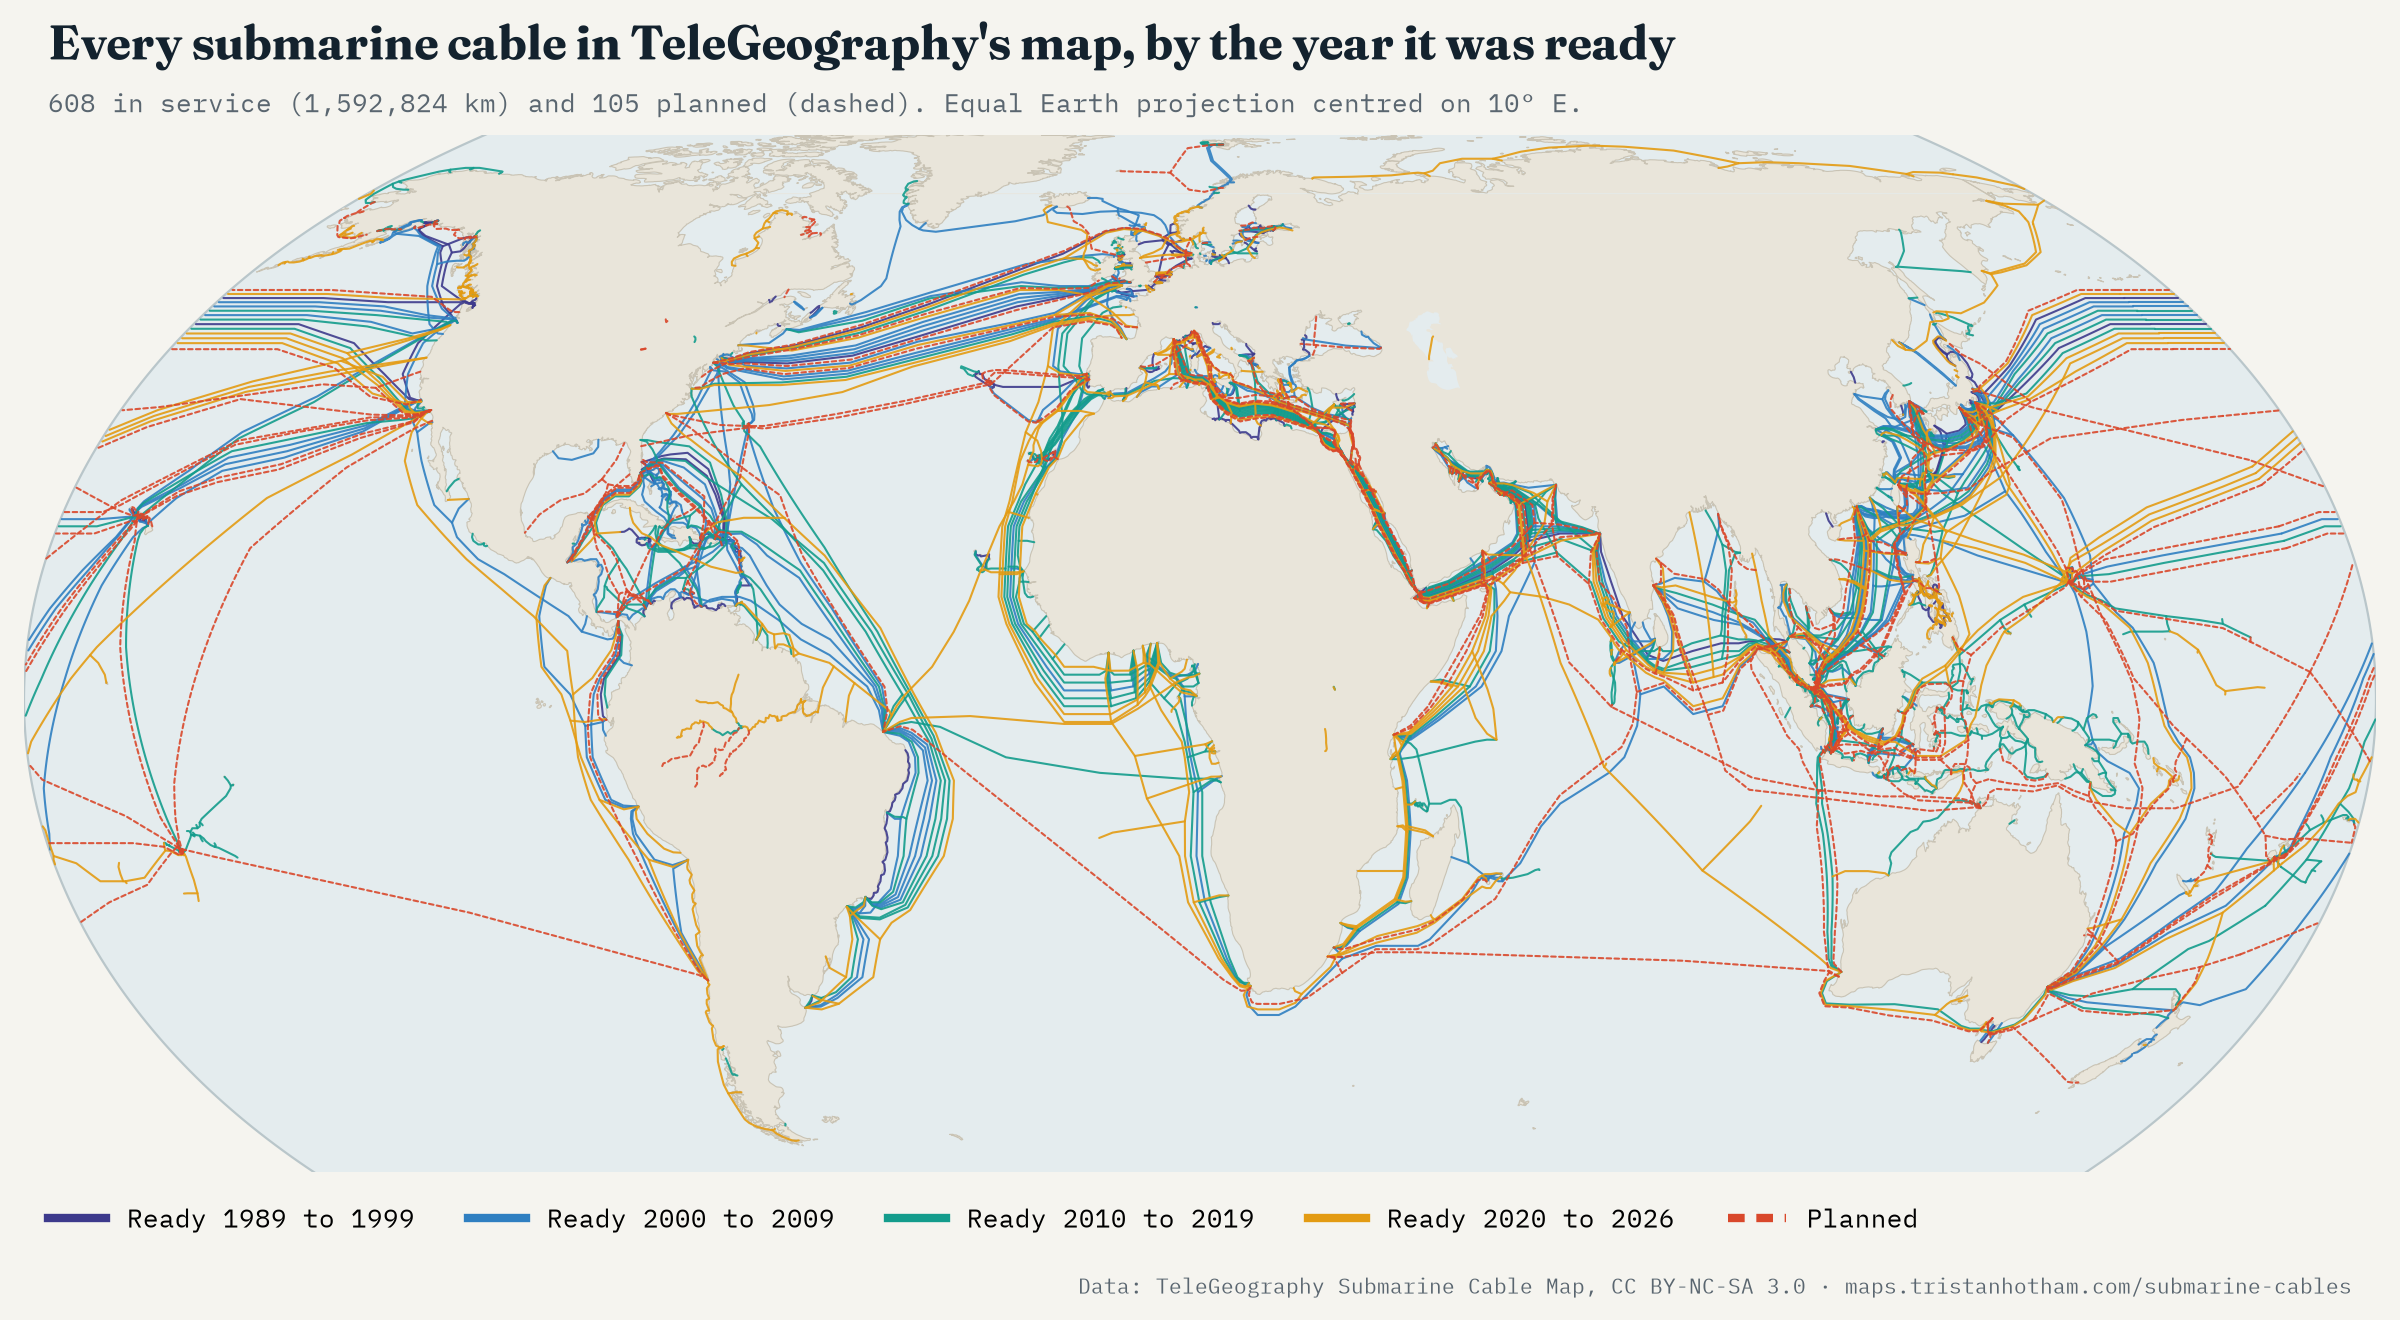
\includegraphics[width=\textwidth]{fig_world.png}\caption{Every cable in TeleGeography's map, coloured by the decade it was ready for service; planned cables dashed.}\label{fig:world}\end{figure}

\subsection{When each cable was laid}
The oldest cables still in service date from 1989, and 113 cables from the 1990s are still in use (Figure~\ref{fig:timeline}). The dot-com boom stands out: 74 of today's cables came into service in 1999 to 2001, with 271,123 km between them, 17\% of all the length in service. 2001 remains the year with the most kilometres (121,657 km). The bust that followed left only 31 cables ready in 2002 to 2004. The count recovered through the 2010s and peaked in 2023 with 32 new cables; 49 are planned for 2027, the largest number for any year in the record. Cables have grown longer: the median length is 230 km for 1990s cables still in service, 548 km for the 2010s, 830 km for the 2020s and 2,569 km for planned cables. Cables ready since 2016 account for 46\% of the length in service.

\begin{figure}[tbp]\centering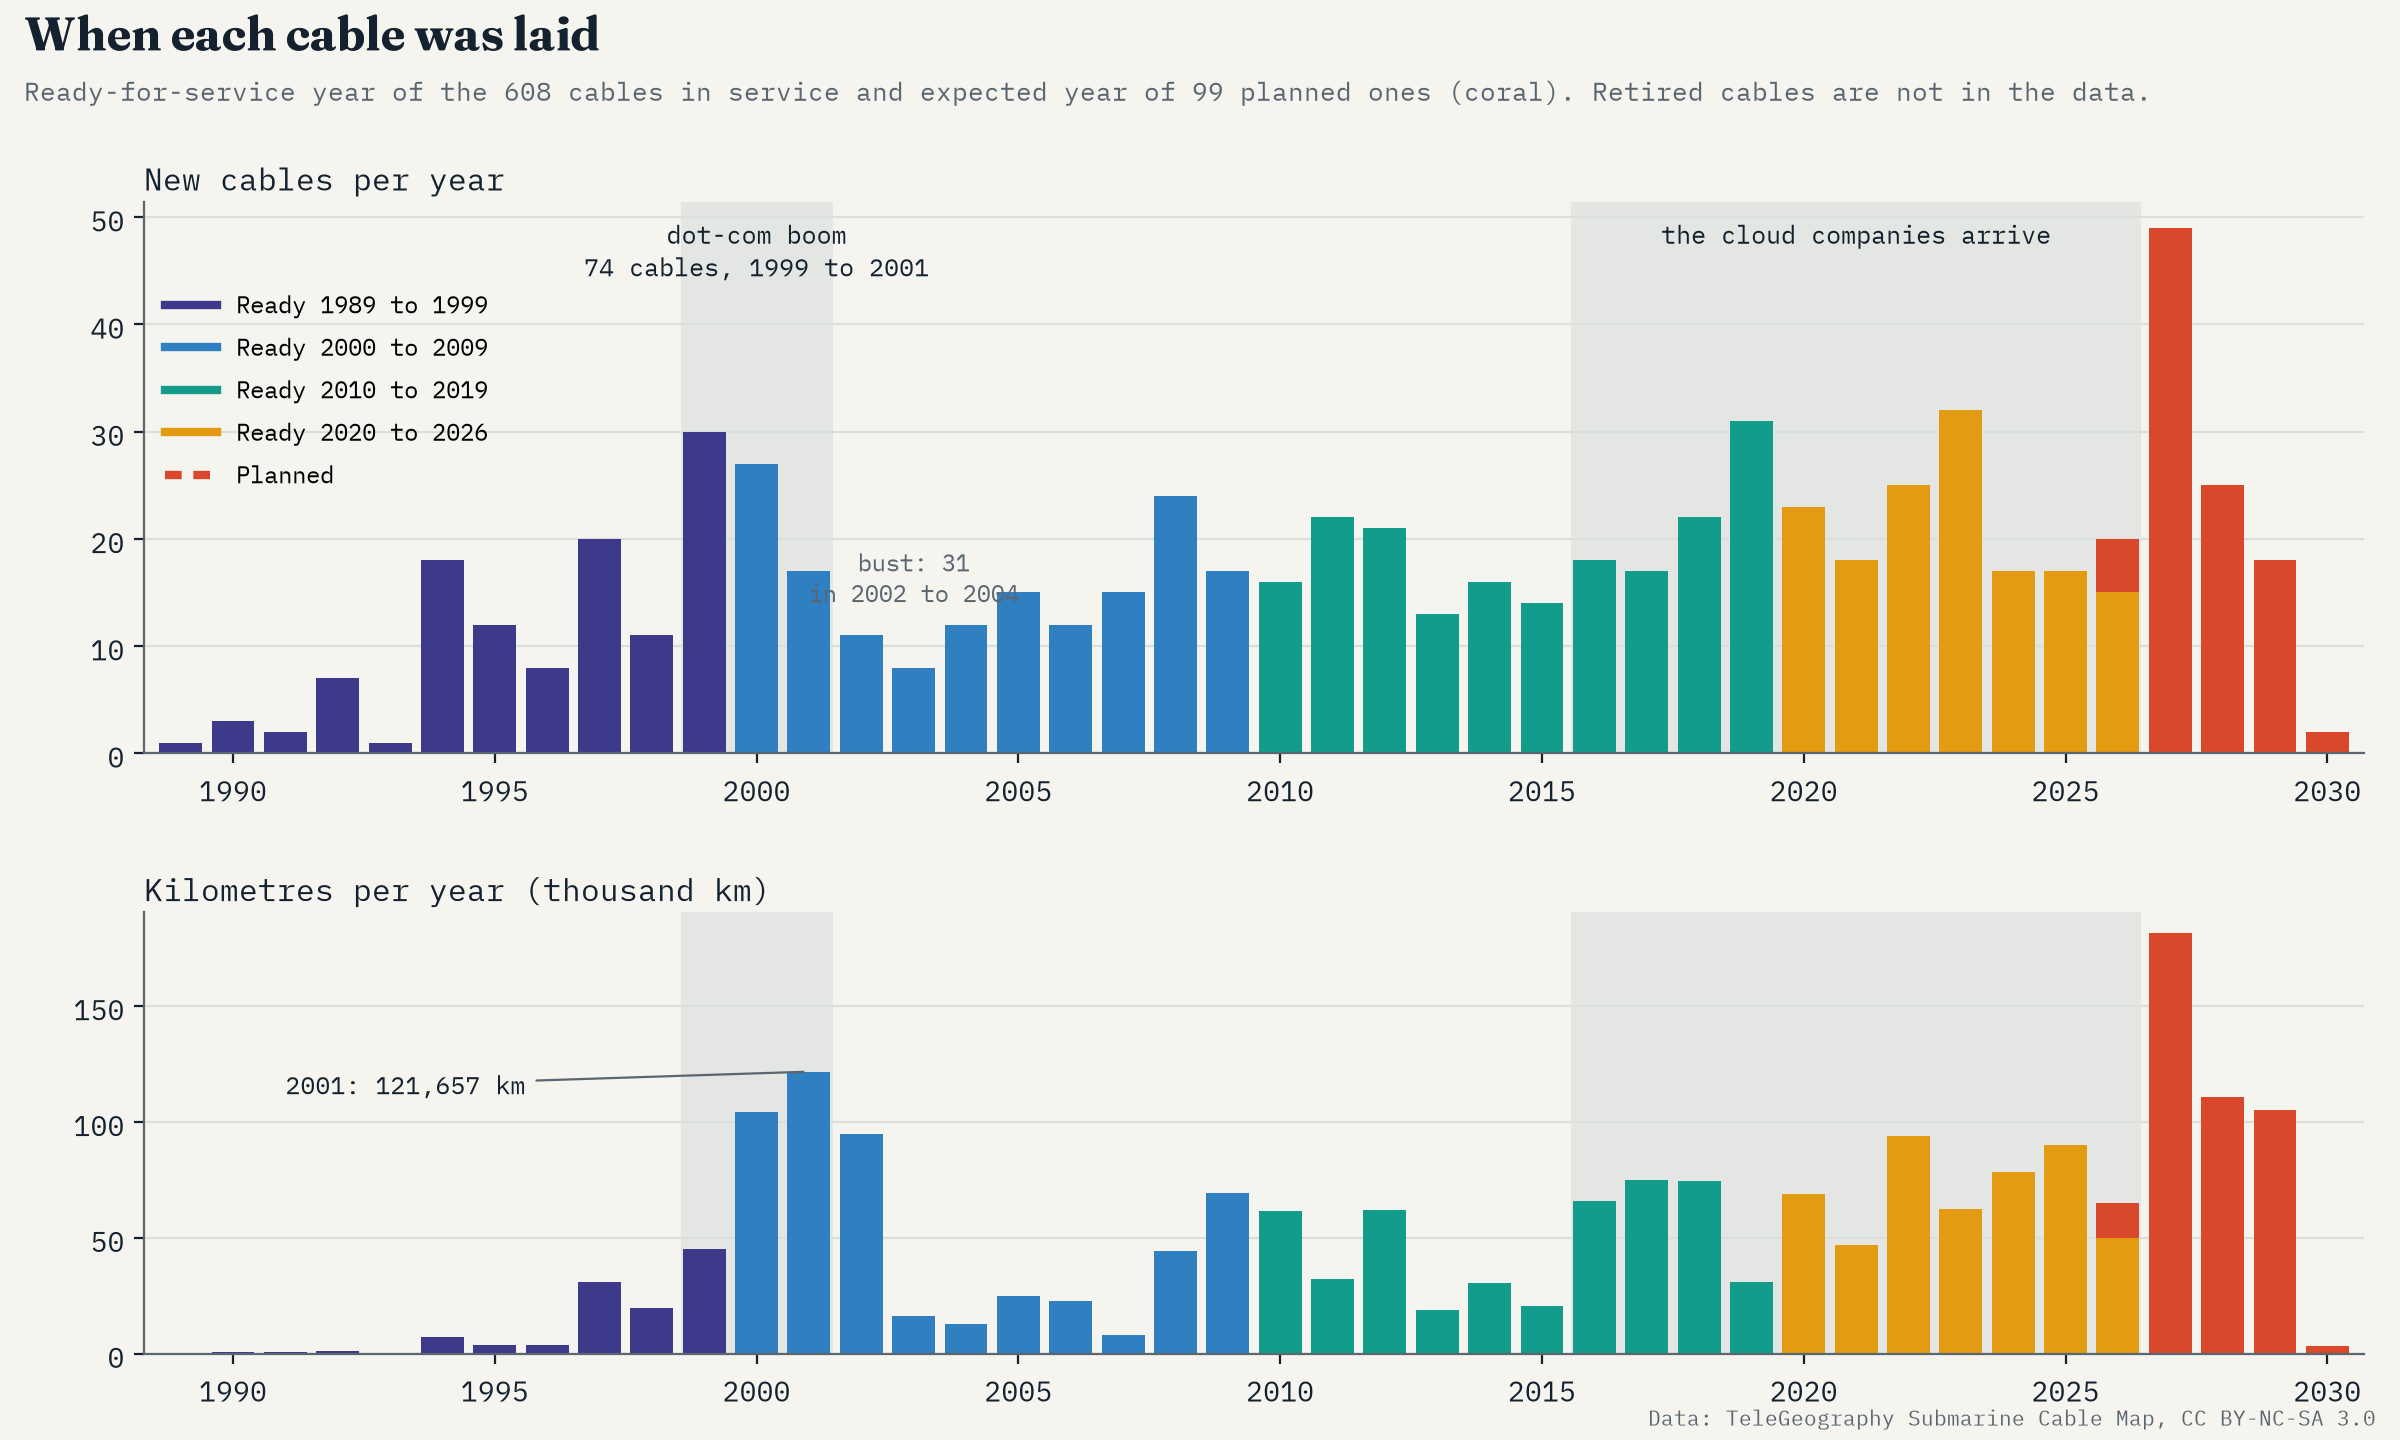
\includegraphics[width=\textwidth]{fig_timeline.png}\caption{New cables and kilometres by ready-for-service year. Coral: planned cables by expected year. The 1990s bars count only cables still in service.}\label{fig:timeline}\end{figure}

\subsection{Who owns the new cables}
Early cables were owned by consortia of telecommunications companies; the record's largest club, SAT-3/WASC, has 33 owners. The four cloud and content companies first appear as owners in 2010 (Unity). Their share of new length rose from zero before 2010 to 9\% in 2010 to 2014, 24\% in 2015 to 2019 and 50\% in 2020 to 2026; they part-own 29 of the 105 planned cables and 55\% of the planned length (Figure~\ref{fig:hyper}). Of the 62 cables with one of them as an owner, 31 have no other owner, 22 of them planned. Google appears in 37 cables (23 alone), Meta in 21, Microsoft in 8 and Amazon in 6.

\begin{figure}[tbp]\centering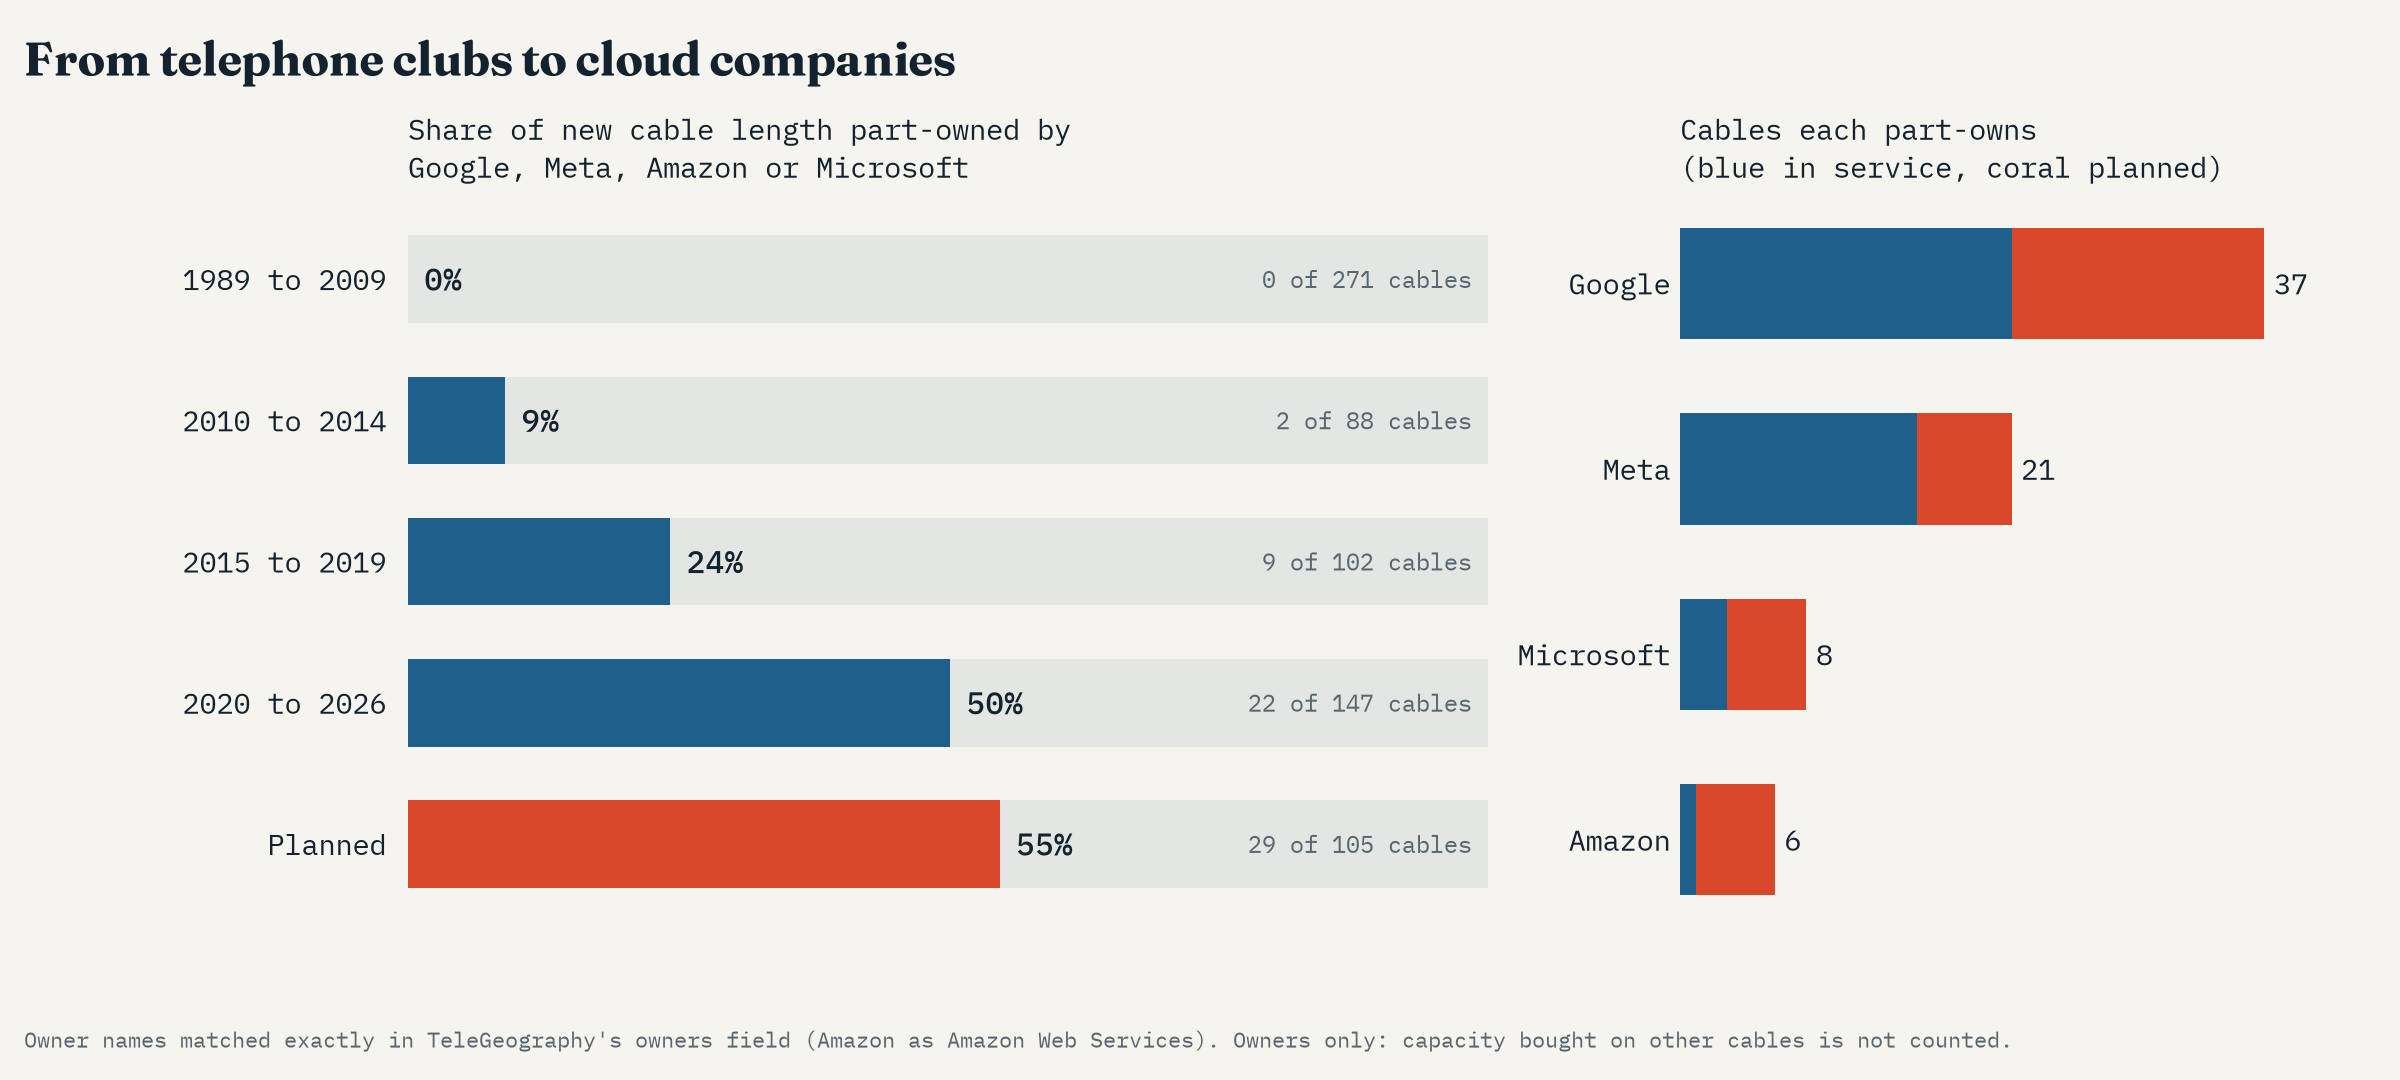
\includegraphics[width=\textwidth]{fig_hyperscalers.png}\caption{Left: share of new cable length part-owned by Google, Meta, Amazon or Microsoft by period. Right: cables each company part-owns.}\label{fig:hyper}\end{figure}

\subsection{Choke points}
Table~\ref{tab:choke} and Figure~\ref{fig:choke} give the counts. Among straits, the Strait of Sicily is the busiest (18 cables in service), followed by the Red Sea at 20° N (13), the Bab el-Mandeb (12), the Luzon Strait (10) and the Strait of Malacca (10). The 12 cables through the Bab el-Mandeb have a combined length of 217,777 km, 14\% of all cable length in service, and 4 more are planned: the Red Sea corridor remains the main route between Europe and Asia, and 9 cables cross Egypt overland to reach the Mediterranean (Figure~\ref{fig:redsea}). The Strait of Gibraltar (3) and the western English Channel (5) are not choke points in this sense: transatlantic cables land on the Atlantic coasts of Europe, and most cables from Asia come ashore within the Mediterranean, at Marseille (12 cables), in Italy and elsewhere.

Among hubs, Singapore has 38 cables in service within 35 km, with 14 planned; then the Boso peninsula south of Tokyo (20), Fujairah (15), Guam (15), Hong Kong (14) and Cornwall (14). The grid (Figure~\ref{fig:density}) confirms these: its busiest cell, off Sakra Island, Singapore, is crossed by 38 cables, then cells off Chikura, Japan (18) and Fujairah, United Arab Emirates (15).

\begin{table}[tbp]\centering\small\caption{Cables through each choke point: in service, planned, and the combined length of the cables in service that pass (km).}\label{tab:choke}\begin{tabular}{lrrr}\toprule Choke point & In service & Planned & Combined km\\\midrule
\multicolumn{4}{l}{\textit{Straits and corridors}}\\
Strait of Sicily & 18 & 5 & 189,713\\
Red Sea (at 20° N) & 13 & 4 & 207,940\\
Bab el-Mandeb & 12 & 4 & 217,777\\
Luzon Strait & 10 & 2 & 133,110\\
Strait of Malacca & 10 & 2 & 88,227\\
Egypt crossing (Suez) & 9 & 3 & 170,511\\
Strait of Hormuz & 5 & 2 & 86,170\\
Western English Channel & 5 & 0 & 42,463\\
Strait of Gibraltar & 3 & 0 & 16,729\\
\multicolumn{4}{l}{\textit{Hub areas}}\\
Singapore & 38 & 14 & 298,156\\
Chikura and the Boso peninsula, Japan & 20 & 4 & 246,994\\
Fujairah and the Gulf of Oman & 15 & 1 & 198,502\\
Guam & 15 & 6 & 156,303\\
Hong Kong & 14 & 2 & 171,067\\
Cornwall (Bude and Porthcurno) & 14 & 0 & 137,370\\
New York and New Jersey & 13 & 3 & 118,213\\
Mumbai & 12 & 4 & 181,538\\
Marseille & 12 & 4 & 152,234\\
South Florida & 11 & 4 & 102,580\\
Hawaii & 10 & 6 & 98,446\\
Fortaleza & 9 & 1 & 126,021\\
\bottomrule\end{tabular}\end{table}

\begin{figure}[tbp]\centering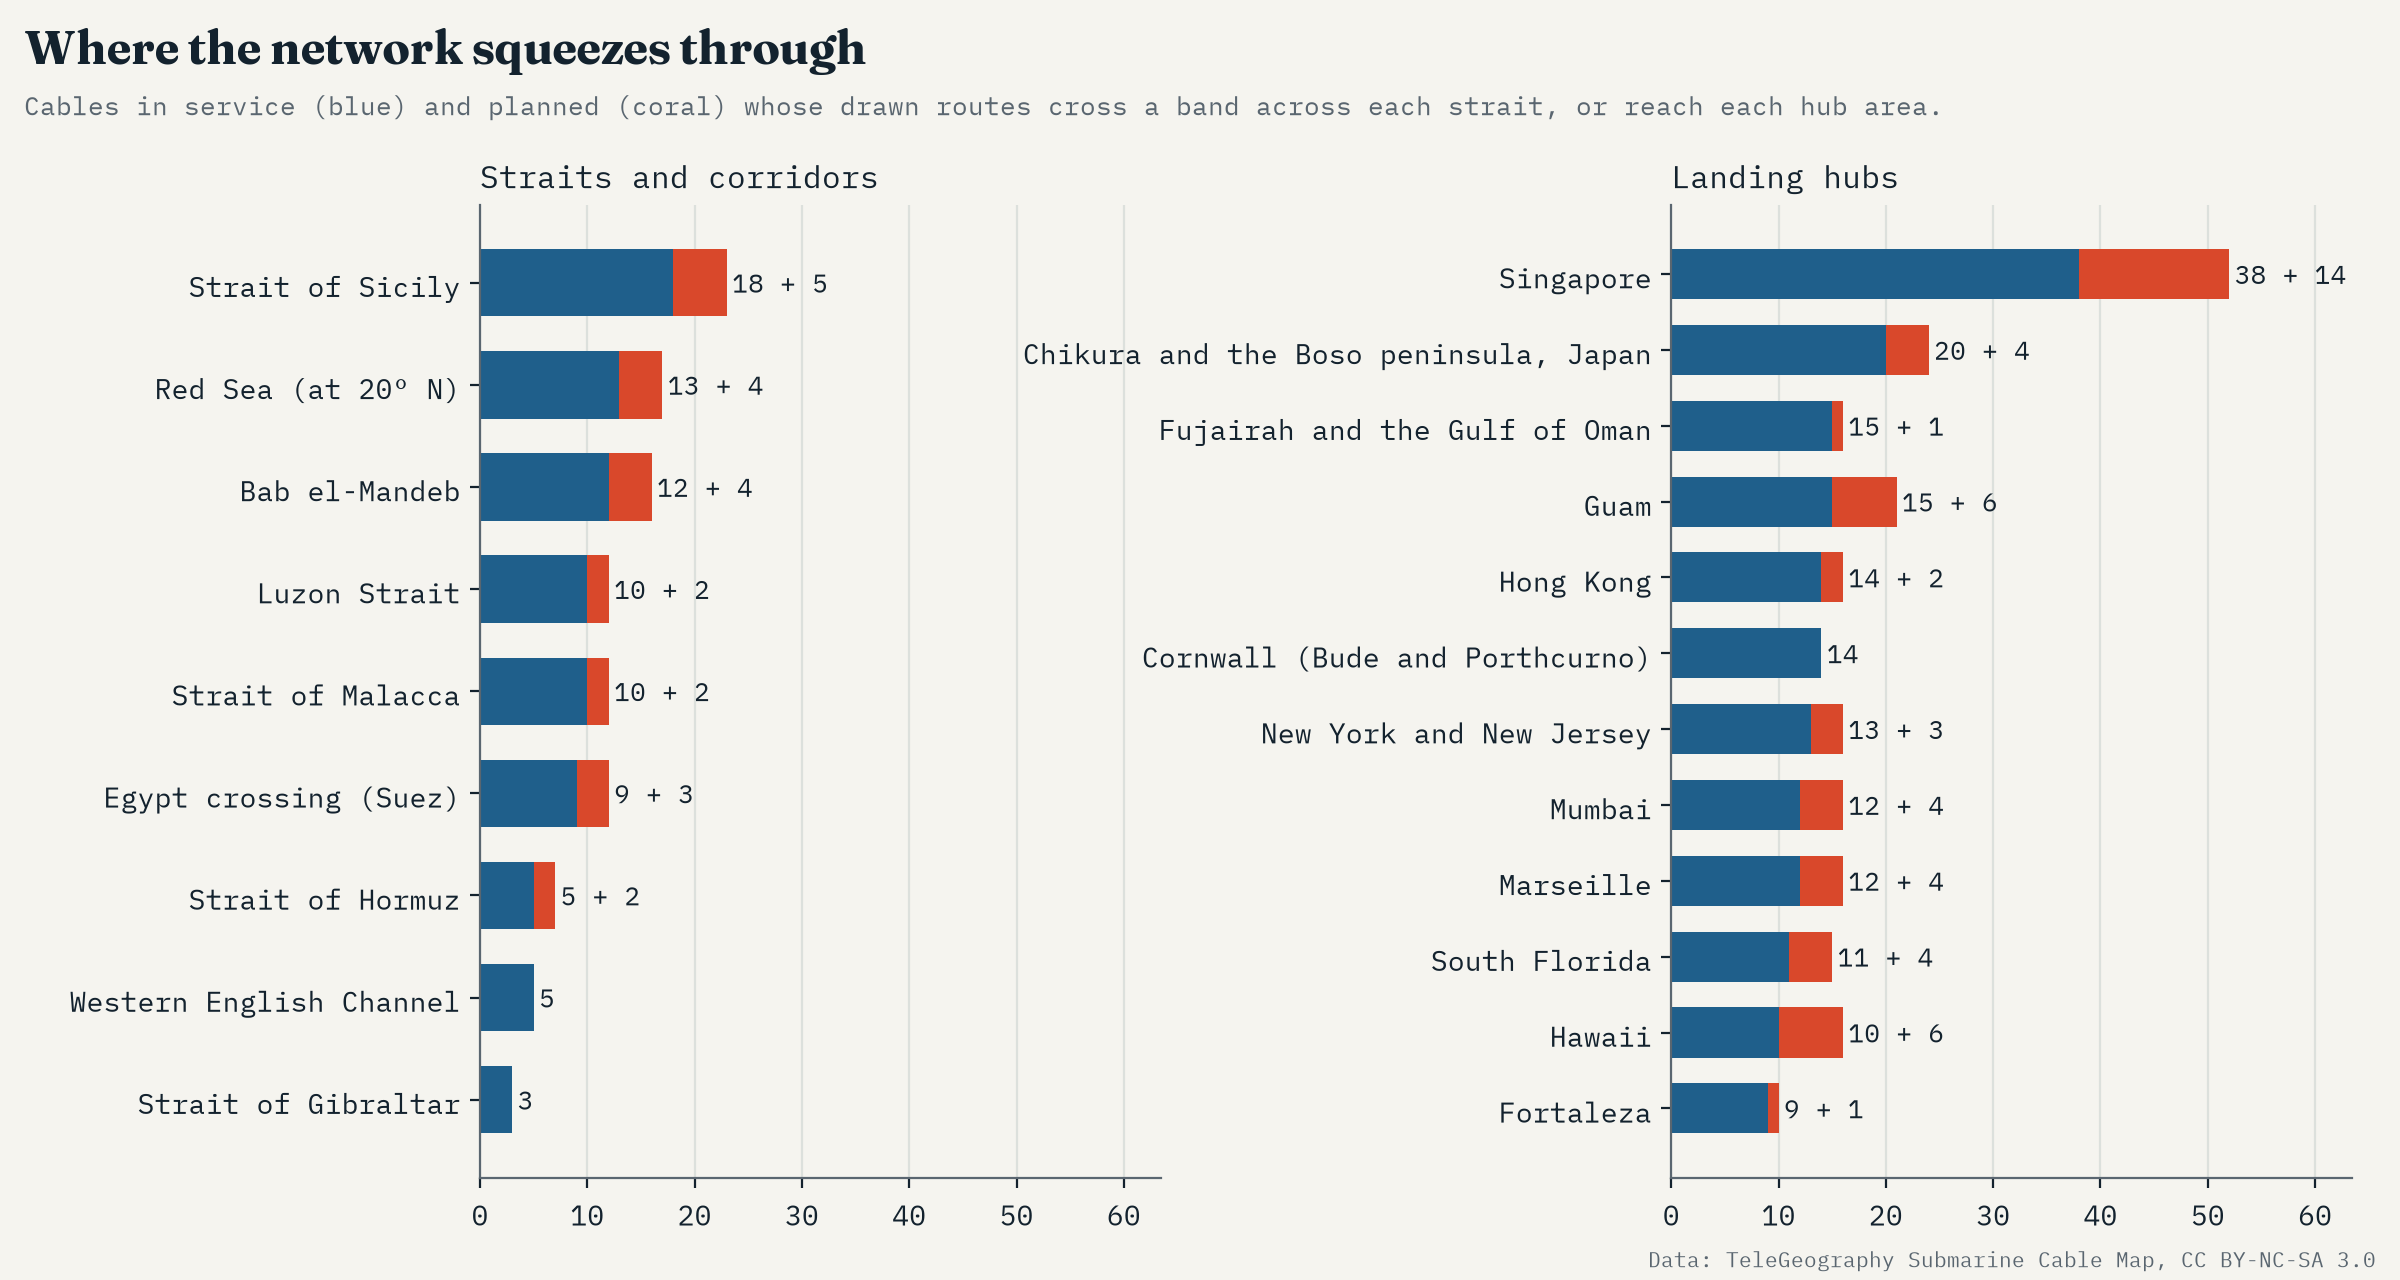
\includegraphics[width=\textwidth]{fig_chokepoints.png}\caption{Cables in service and planned through each strait or corridor and reaching each hub area.}\label{fig:choke}\end{figure}

\begin{figure}[tbp]\centering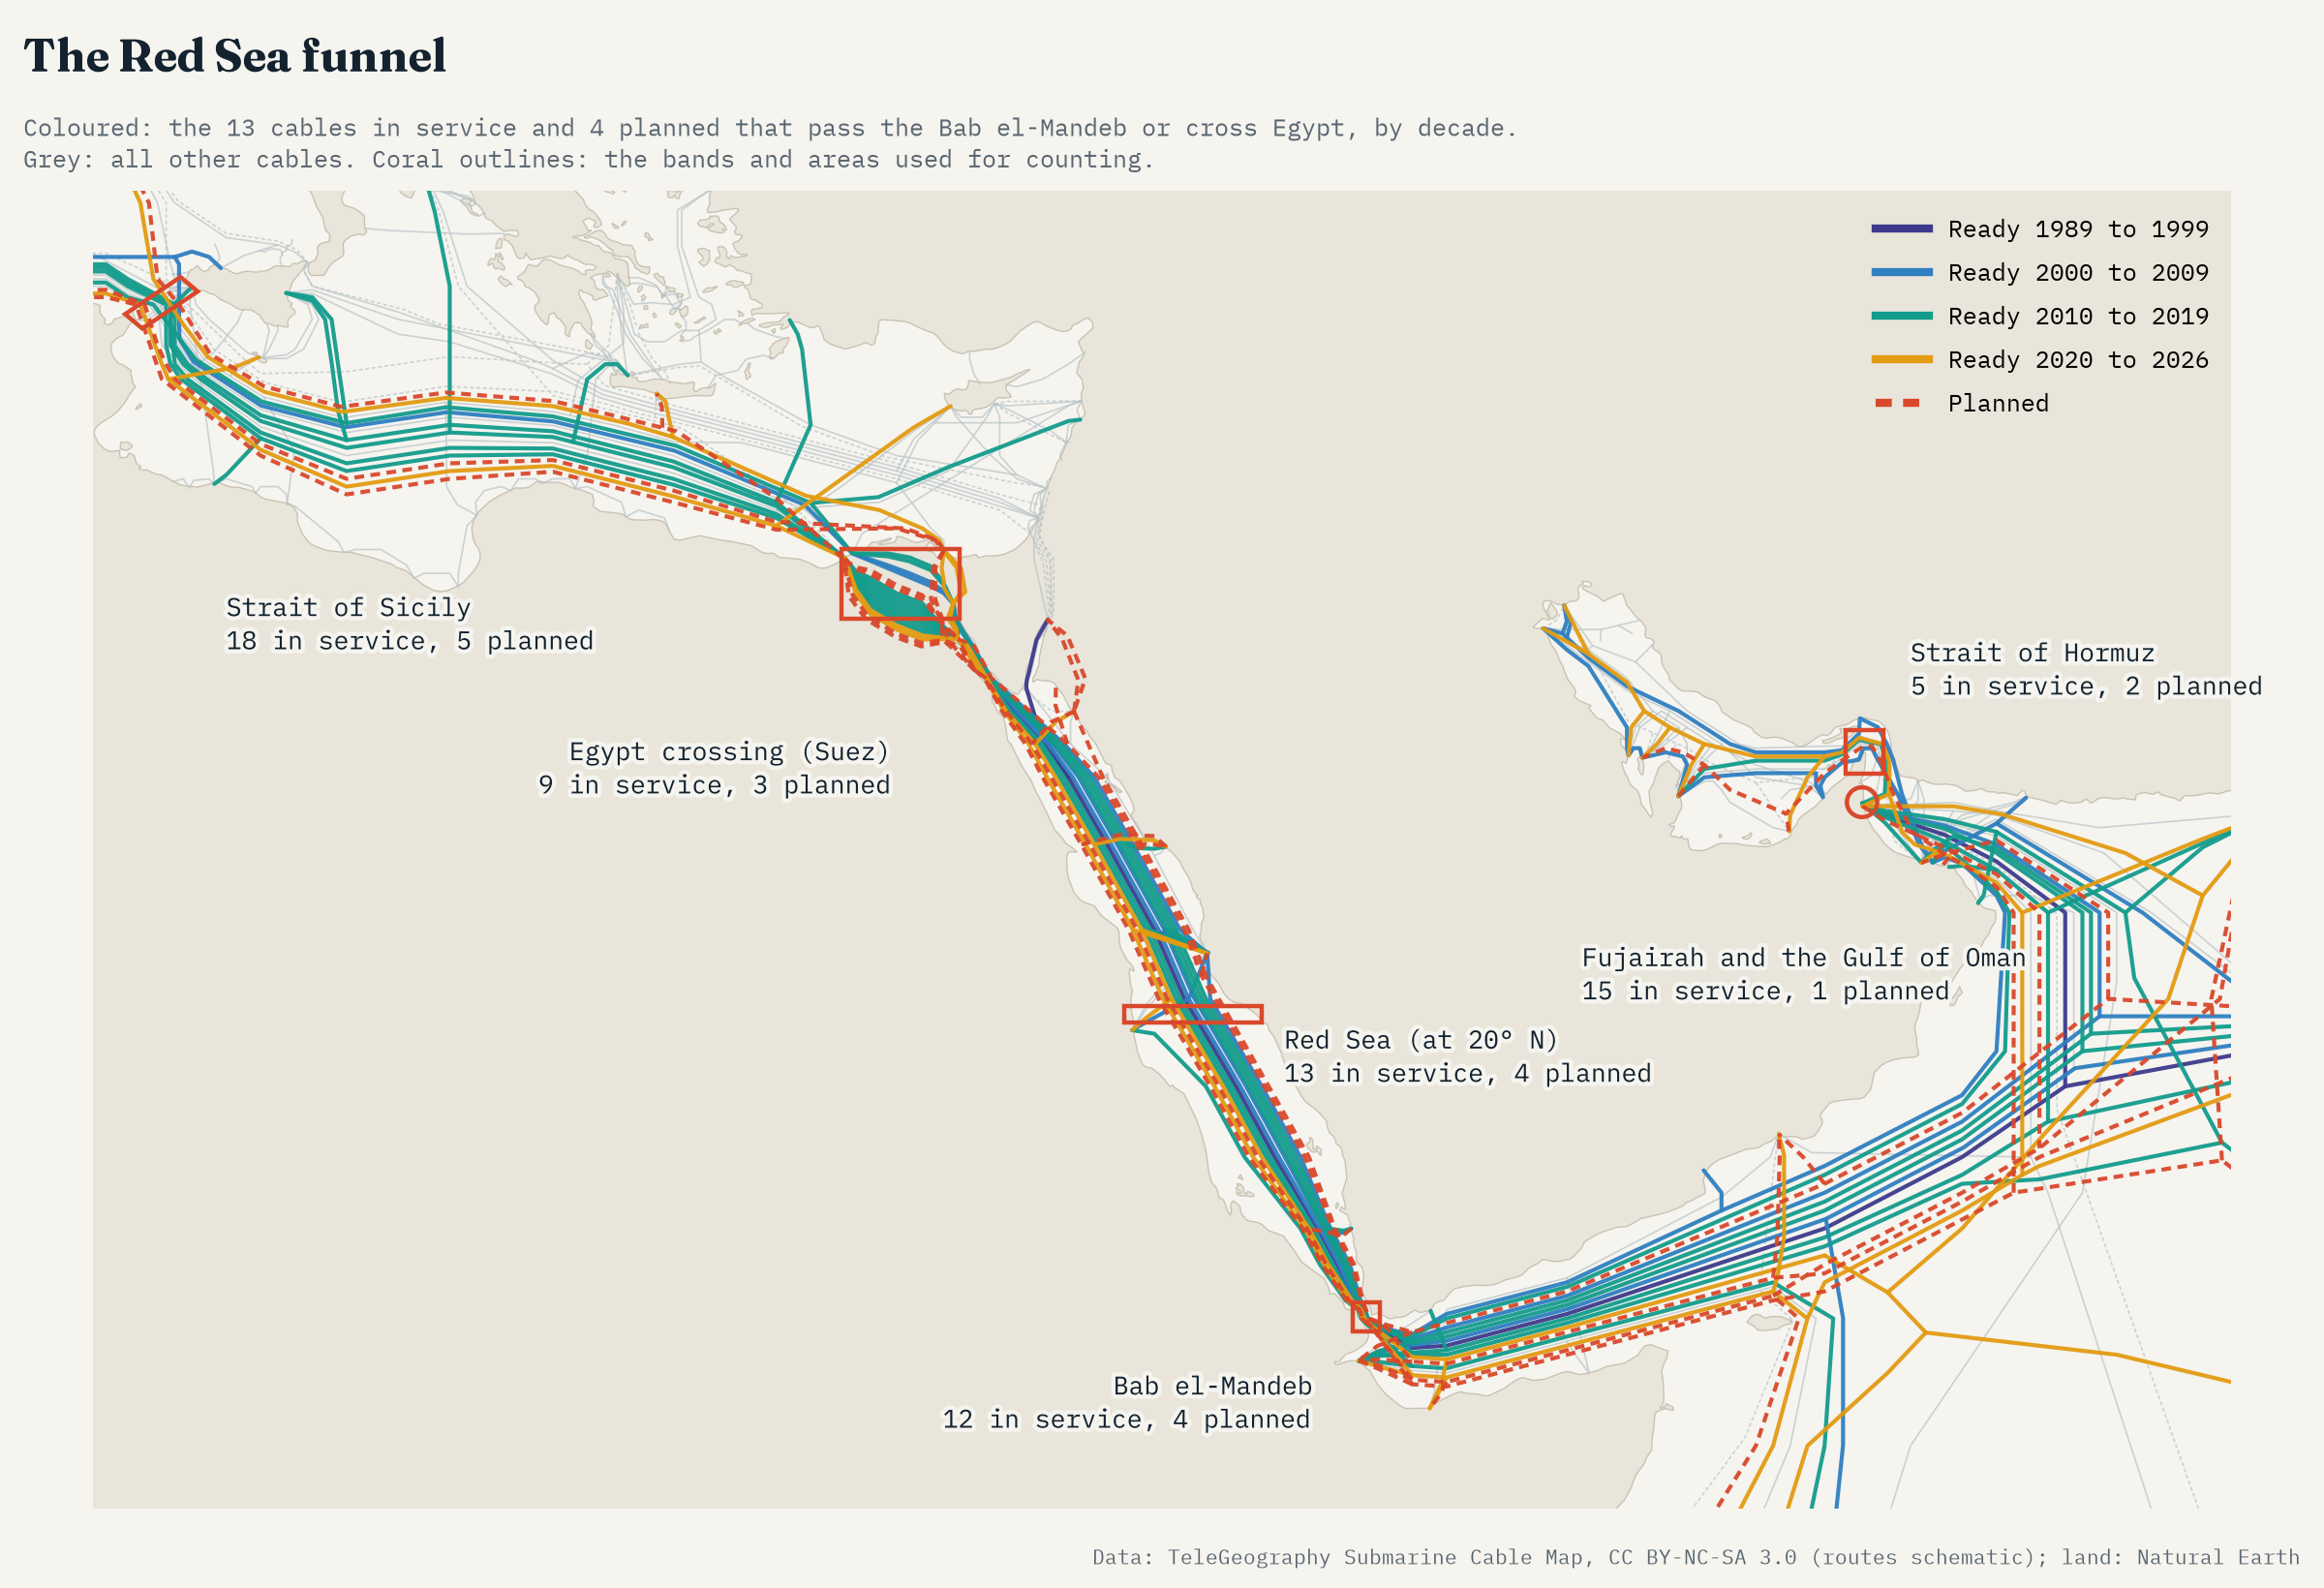
\includegraphics[width=\textwidth]{fig_redsea.png}\caption{The Red Sea corridor. Coloured: cables that pass the Bab el-Mandeb or cross Egypt; grey: all other cables; coral outlines: counting bands and areas.}\label{fig:redsea}\end{figure}

\begin{figure}[tbp]\centering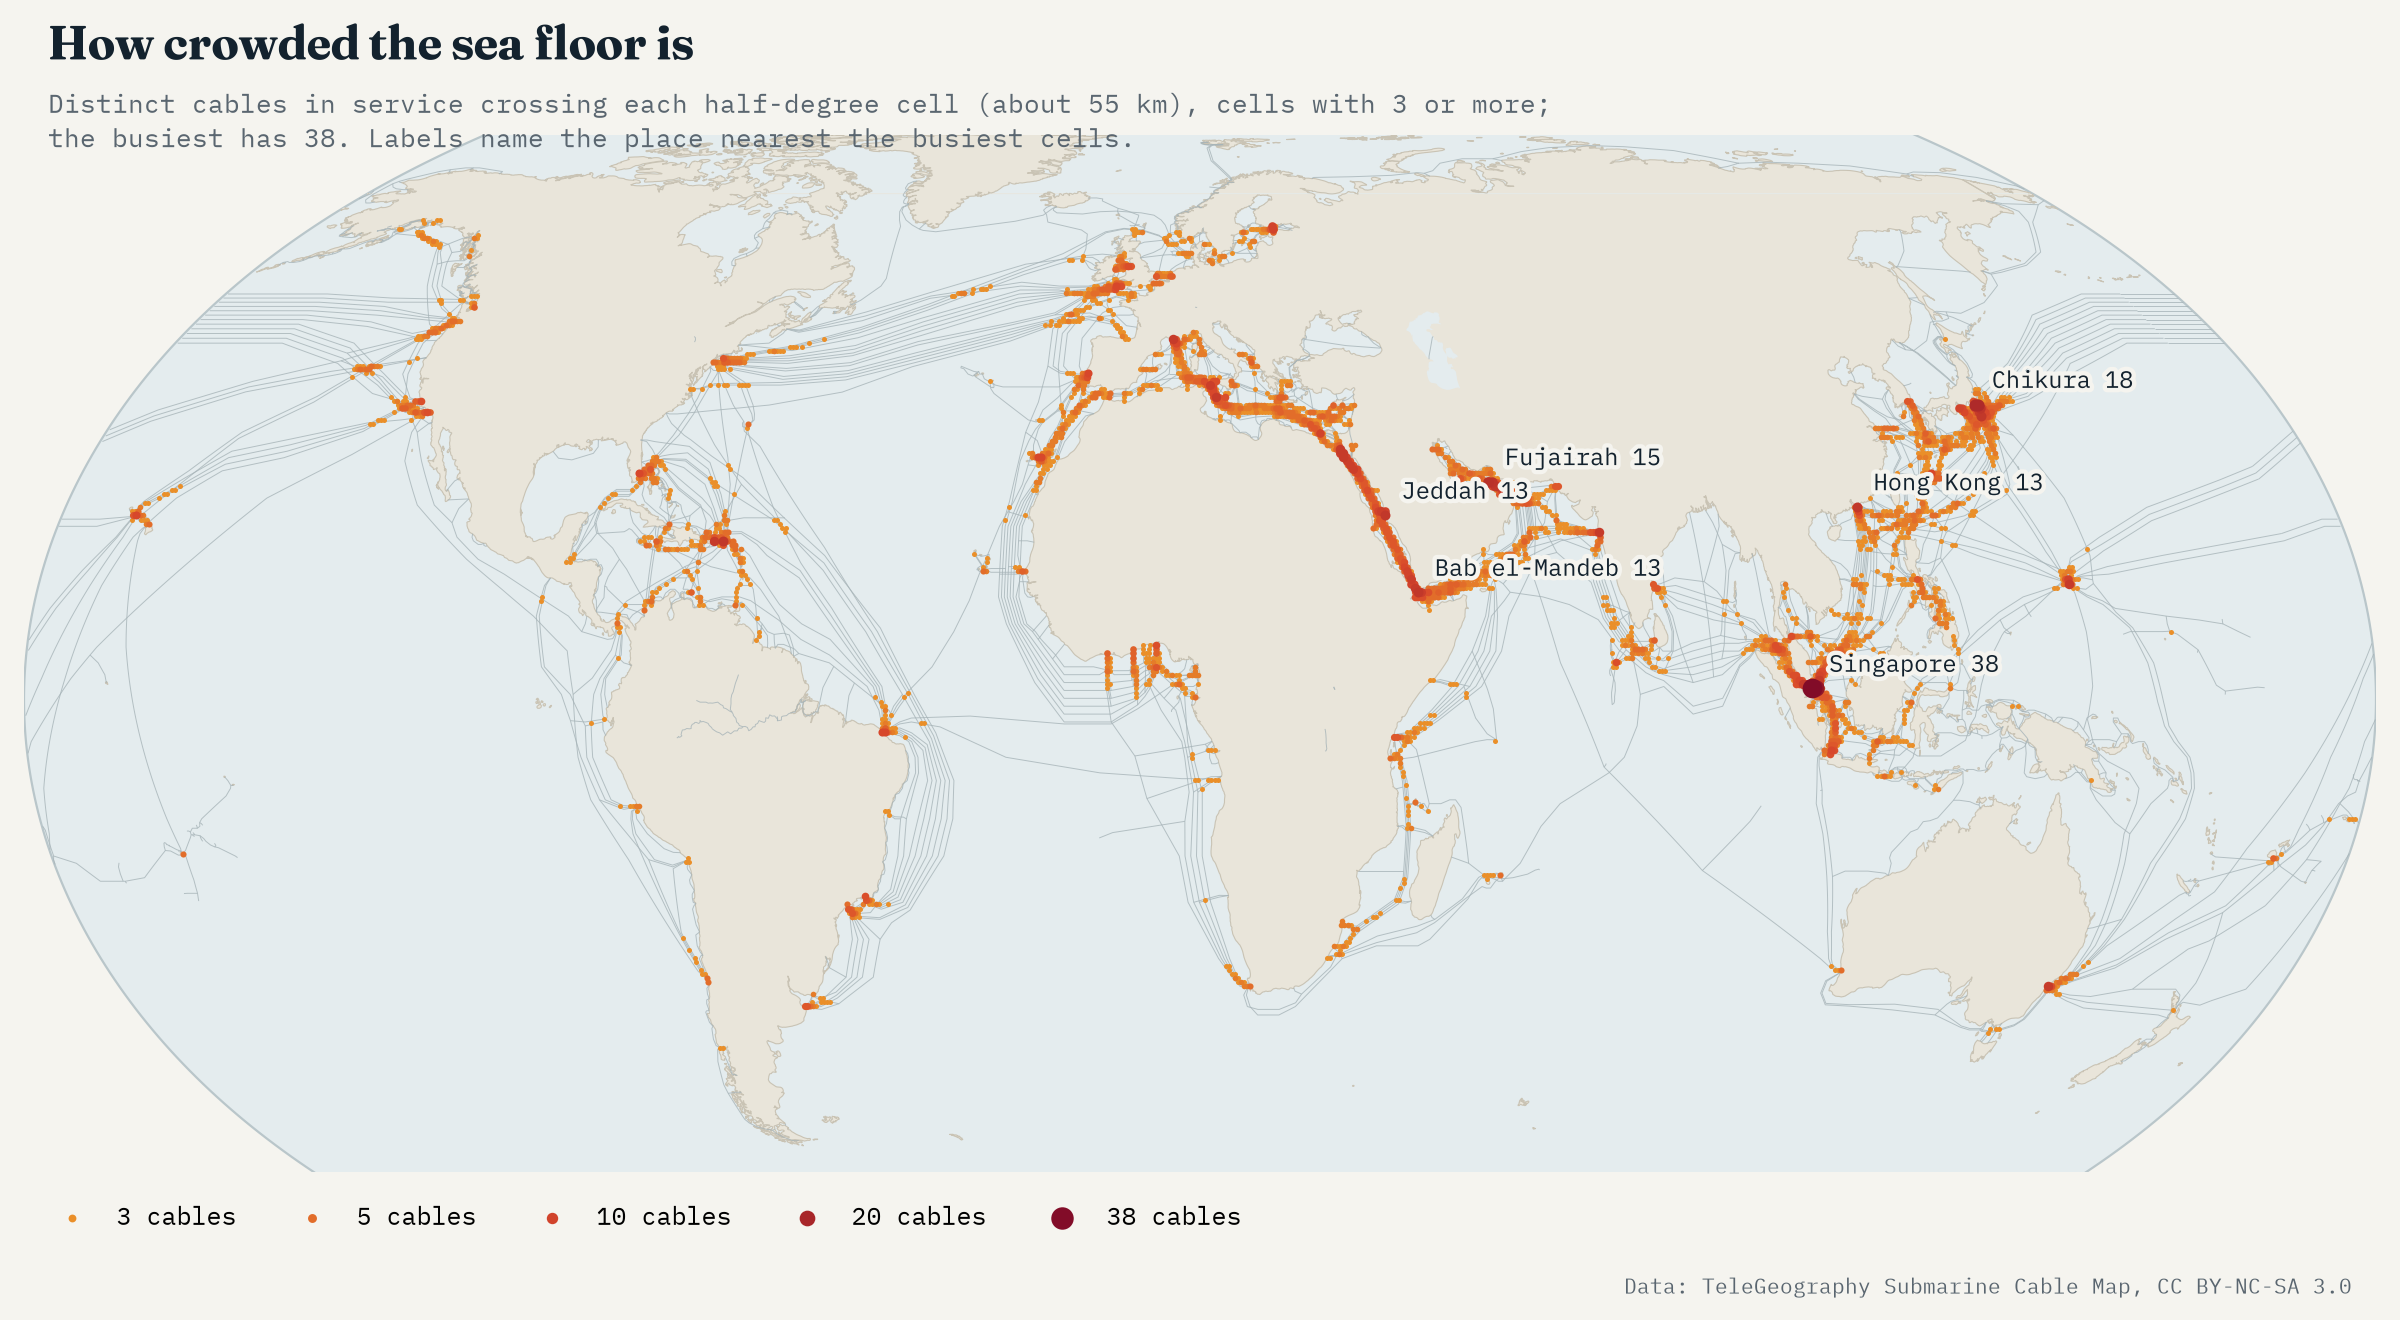
\includegraphics[width=\textwidth]{fig_density.png}\caption{Distinct cables in service crossing each half-degree cell (cells with three or more).}\label{fig:density}\end{figure}

\subsection{Most and least connected}
The United States has the most international cables in service (59), then the United Kingdom (51) and Singapore (34); 30 countries and territories have ten or more (Figure~\ref{fig:connected}). 29 have exactly one. 12 of these have land borders and can also be reached overland; the other 17 are islands with no land border, mostly small territories in the Pacific, Atlantic, Indian Ocean and Caribbean, plus Greenland. 3 of them have a further cable planned. Tuvalu appears only on a planned cable, and Timor-Leste only on a domestic one. Among coastal sovereign states, El Salvador, Eritrea, Montenegro, North Korea and Turkmenistan do not appear in the data at all. Tonga's experience in 2022 shows what one cable means: when its only international cable was cut, the islands were largely cut off for weeks. In the 2026 record Tonga also lands on Hawaiki, whose ready-for-service year (2018) is that of the main system; the record does not date branches separately.

At the scale of landing stations, 1,312 of the 1,792 landing points in service (73\%) serve a single cable, and 8 serve ten or more; the busiest are Batam, Indonesia and Tuas, Singapore (14 each).

\begin{figure}[tbp]\centering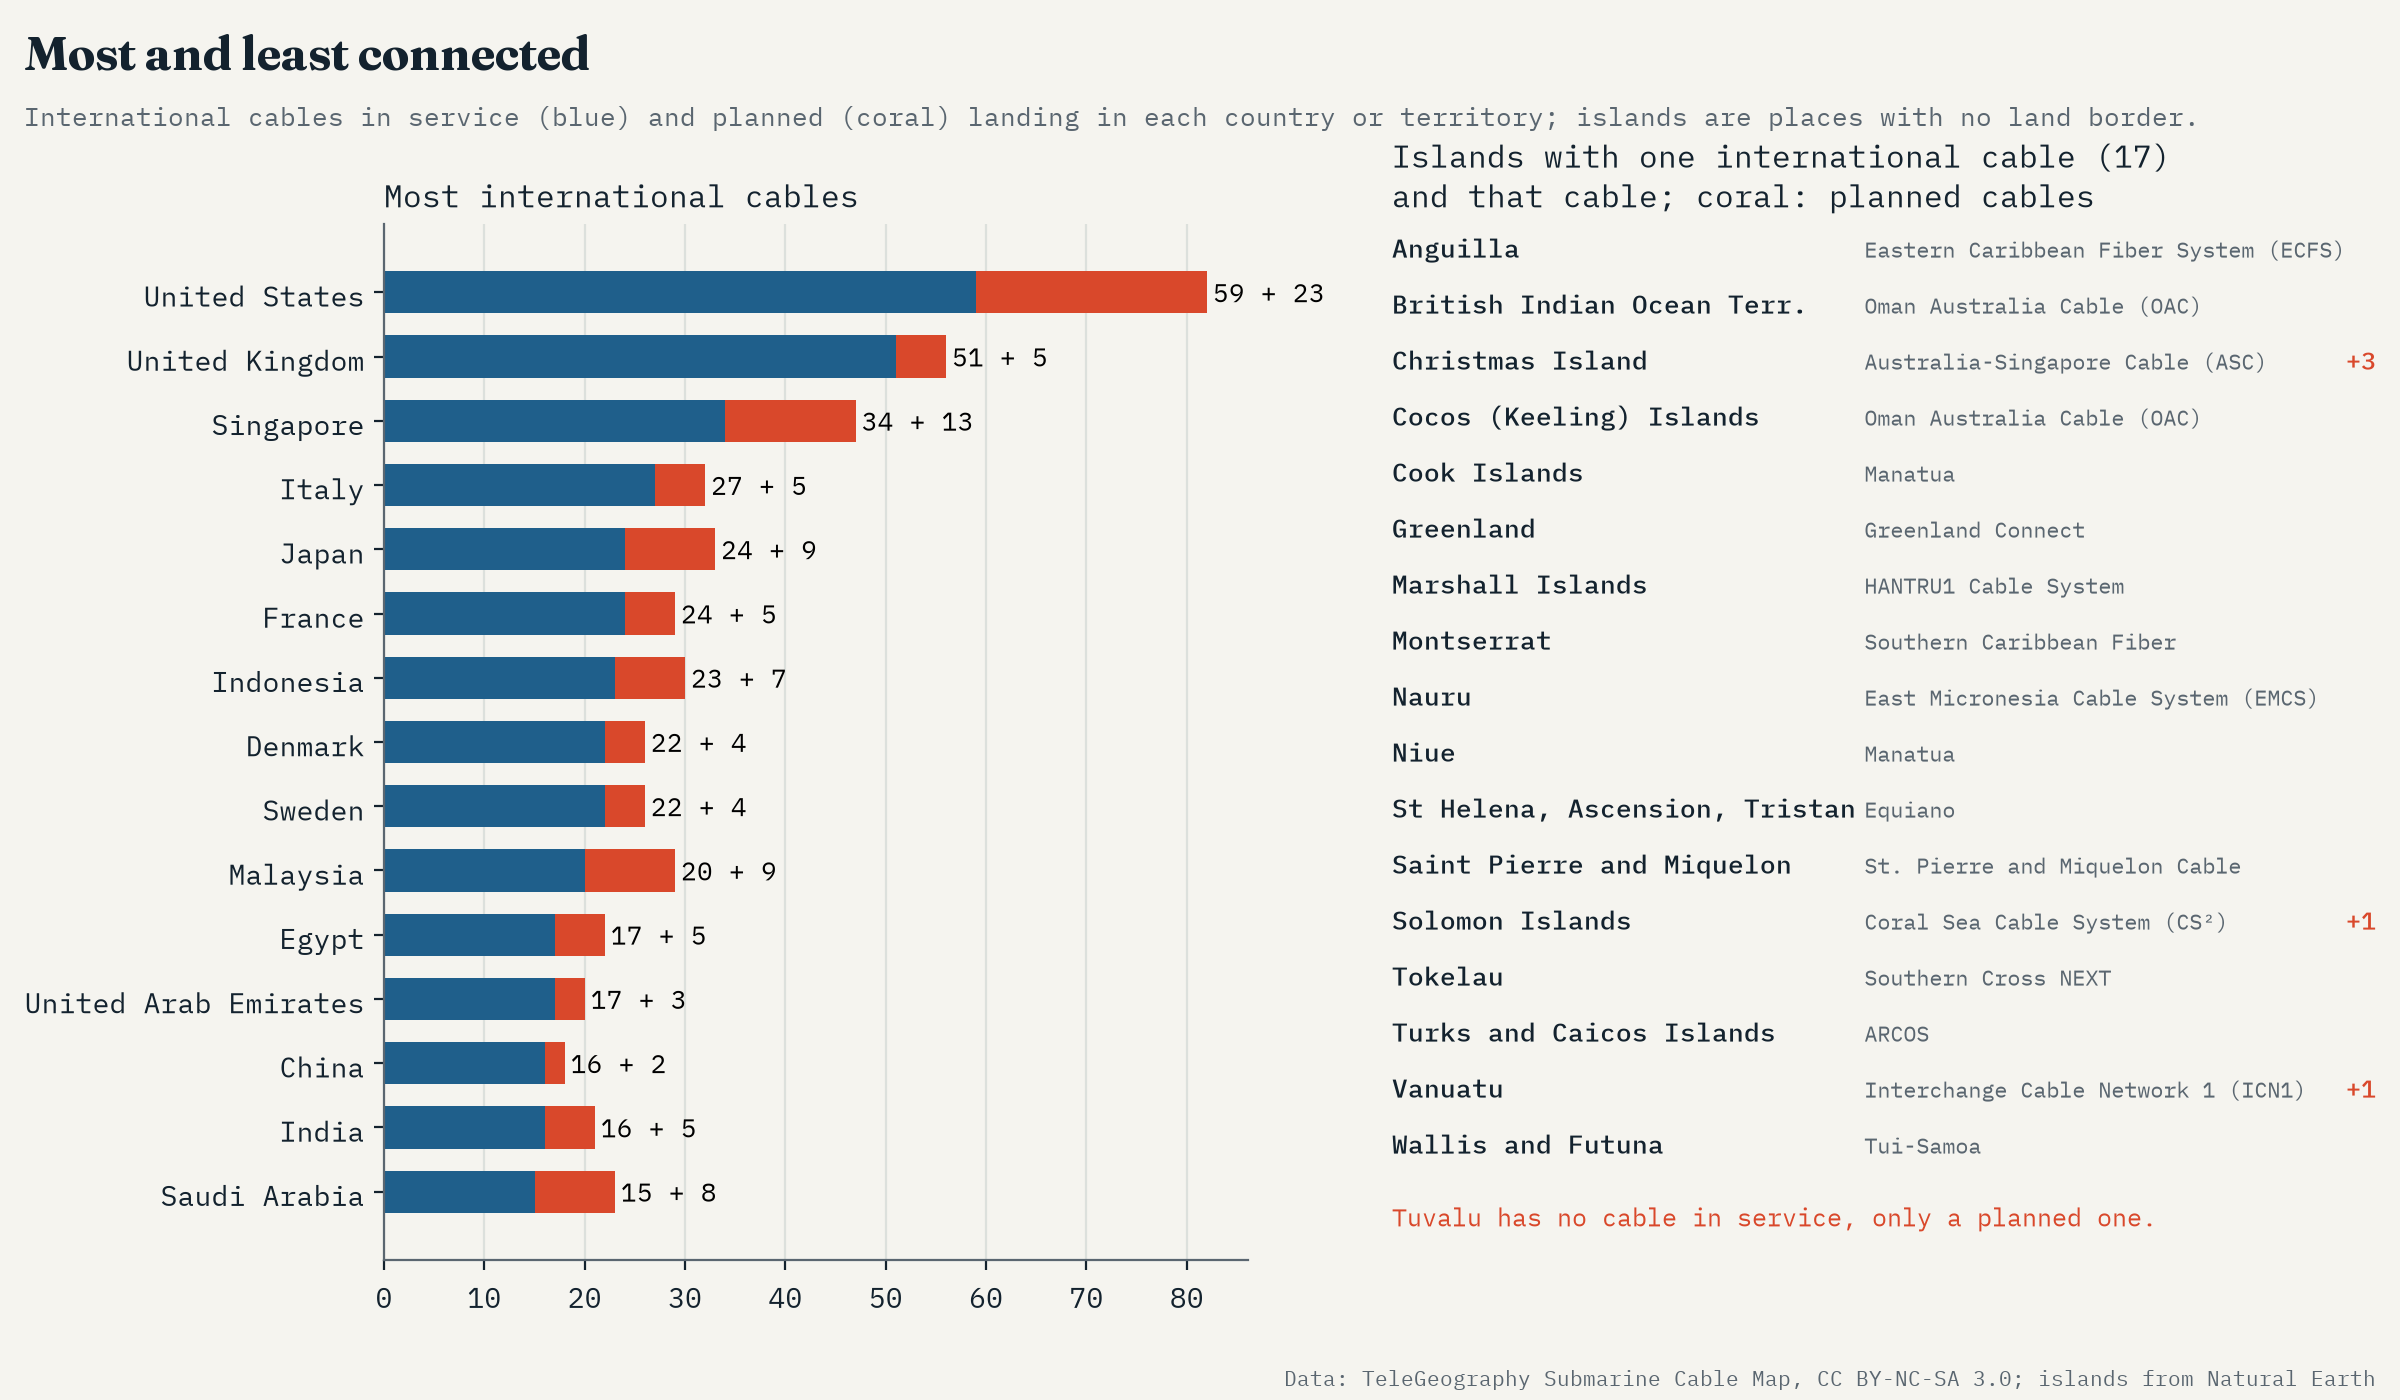
\includegraphics[width=\textwidth]{fig_connected.png}\caption{Left: countries and territories with the most international cables. Right: islands with a single international cable.}\label{fig:connected}\end{figure}

\section{Limitations}
The record omits retired cables, so the early years undercount what was laid. It has no capacities: a 1990s cable with a few gigabits per second counts the same as a new cable with hundreds of terabits. Routes are schematic, so counts near the edge of a band or area can be off by one or two, and the choice of bands and areas is mine; the grid offers a check that does not depend on it. Owners are as TeleGeography lists them, and capacity agreements are invisible. The island classification uses land borders as drawn by Natural Earth and ignores land cables, causeways and satellite links. Nothing here assesses the security of any particular cable, and counts of cables through a strait are not a measure of risk on their own: depth, seabed, shipping and repair capacity all matter \citep{carter2009}.

\section*{Data availability}
Derived data (cables, landing points, countries, choke points, grid, timeline and the full results) and all code are at \url{https://github.com/Tristan-Hotham/submarine-cables} and archived with this paper. Derived data, figures and text are shared under CC BY-NC-SA 4.0, a later version of the licence of TeleGeography's data (CC BY-NC-SA 3.0), which the 3.0 licence permits for adaptations; the code is MIT licensed.

\section*{AI statement}
I wrote the text, with drafting and editing assistance from Claude (Anthropic), which also helped prepare the analysis code. I reviewed and checked all text and results.

\begin{thebibliography}{99}
\bibitem[Burnett et al.(2014)]{burnett2014} Burnett, D.R., Beckman, R.C. and Davenport, T.M. (eds.) (2014) \emph{Submarine Cables: The Handbook of Law and Policy}. Leiden: Martinus Nijhoff.
\bibitem[Carter et al.(2009)]{carter2009} Carter, L., Burnett, D., Drew, S., Marle, G., Hagadorn, L., Bartlett-McNeil, D. and Irvine, N. (2009) \emph{Submarine Cables and the Oceans: Connecting the World}. UNEP-WCMC Biodiversity Series 31. ICPC and UNEP-WCMC.
\bibitem[Natural Earth(2026)]{naturalearth} Natural Earth (2026) 1:10m and 1:50m cultural and physical vectors. Public domain. \url{https://www.naturalearthdata.com/}
\bibitem[Starosielski(2015)]{starosielski2015} Starosielski, N. (2015) \emph{The Undersea Network}. Durham, NC: Duke University Press.
\bibitem[TeleGeography(2026)]{telegeography} TeleGeography (2026) Submarine Cable Map, API version 3. CC BY-NC-SA 3.0. \url{https://www.submarinecablemap.com/}
\end{thebibliography}
\end{document}
